 %% LyX 2.3.4.2 created this file.  For more info, see http://www.lyx.org/.
%% Do not edit unless you really know what you are doing.
%\documentclass{achemso}
\documentclass[journal=mamobx, layout=twocolumns,manuscript=article]{achemso}

\usepackage[utf8]{inputenc}
\usepackage{geometry}
\geometry{verbose}
\usepackage{xcolor}
\usepackage{verbatim}
\usepackage{multirow}
\usepackage{amsmath}
\usepackage{amsthm}
\usepackage{graphicx}
\usepackage[unicode=true,pdfusetitle,
 bookmarks=false,
 breaklinks=true,pdfborder={0 0 0},pdfborderstyle={},backref=false,colorlinks=true]
 {hyperref}
\usepackage[textsize=small]{todonotes}


\makeatletter

%%%%%%%%%%%%%%%%%%%%%%%%%%%%%% LyX specific LaTeX commands.


\title{Water desalination using polyelectrolyte hydrogel. Gibbs ensemble
modelling}


\author{Mikhail Laktionov}

\affiliation[cuni]{Department of Physical and Macromolecular Chemistry, Faculty of Science,
Charles University in Prague, Czech Republic}


\alsoaffiliation[itmo]{St. Petersburg National Research University of Information Technologies,
Mechanics and Optics, St. Petersburg, Russia.}

\author{Lucie Nová}
\author{Oleg V. Rud}


\affiliation{Department of Physical and Macromolecular Chemistry, Faculty of Science,
Charles University in Prague, Czech Republic}


\alsoaffiliation[imc]{Institute of Macromolecular Compounds of Russian Academy of Sciences,
Saint-Petersburg, Russia}


\email{oleg.rud@natur.cuni.cz}



\abbreviations{MC, MD, RO, FO}


\keywords{polyelectrolye hydrogel, simulation, desalination}

%% Because html converters don't know tabularnewline
\providecommand{\tabularnewline}{\\}


%%%%%%%%%%%%%%%%%%%%%%%%%%%%%% User specified LaTeX commands.
%\usepackage[utf8]{inputenc}
\usepackage{amssymb}
%%%%%%%%%%%%%%%%%%%%%%%%%%%%%% User specified LaTeX commands.
\newcommand{\ie}{\textit{i.~e.} }
\newcommand{\cref}{c^{\ominus}}
%\newcommand{\cs}{c_{s}}
\newcommand{\kT}{k_\mathrm{B}T}
\newcommand{\kB}{k_\mathrm{B}}
\newcommand{\lb}{l_\mathrm{B}}
\newcommand{\NA}{N_{\mathrm{A^-}}}
\newcommand{\muna}{\mu_\mathrm{Na^+}}

\newcommand{\mucl}{\mu_\mathrm{Cl^-}}
\newcommand{\muca}{\mu_\mathrm{Ca^{2+}}}
\newcommand{\muh}{\mu_\mathrm{H^+}}
\newcommand{\mua}{\mu_\mathrm{A^-}}
\newcommand{\muha}{\mu_\mathrm{HA}}
\newcommand{\muoh}{\mu_\mathrm{OH}}

\newcommand{\cna}{c_\mathrm{Na^+}}
\newcommand{\ccl}{c_\mathrm{Cl^-}}
\newcommand{\cca}{c_\mathrm{Ca^{2+}}}
\newcommand{\ch}{c_\mathrm{H^+}}
\newcommand{\cp}{c_\mathrm{p}}
\newcommand{\nna}{n_\mathrm{Na^+}}
\newcommand{\ncl}{n_\mathrm{Cl^-}}
\newcommand{\Nna}{N_\mathrm{Na^+}}
\newcommand{\Ncl}{N_\mathrm{Cl^-}}

\newcommand{\ncleq}{\widetilde{N}_\mathrm{Cl^-}}
\newcommand{\nca}{N_\mathrm{Ca^{2+}}}

\newcommand{\superin}{^\mathrm{in}}
\newcommand{\subin}{_\mathrm{in}}
\newcommand{\subi}{_\mathrm{i}}

\newcommand{\gel}{^\mathrm{gel}}
\newcommand{\tot}{^\mathrm{tot}}
\newcommand{\out}{^{\mathrm{out}}}
\newcommand{\coh}{c_\mathrm{OH}}
\newcommand{\bulk}{^{\mathrm{b}}}
\renewcommand{\H}{\mathrm{H^+}}
\newcommand{\A}{\mathrm{A^-}}
\newcommand{\AH}{\mathrm{AH}}
%%%%%%%%%%%%%%%%%%%%%%%%%%%%%% LyX specific LaTeX commands.
%% A simple dot to overcome graphicx limitations
\newcommand{\lyxdot}{.}
\newcommand{\todoi}[1]{\todo[inline]{#1}}
\setuptodonotes{fancyline, color=blue!30, size=\tiny}

\newcommand{\cl}{\mathrm{Cl^-}}
\newcommand{\br}{\mathrm{Br^-}}
\newcommand{\na}{\mathrm{Na^+}}
\newcommand{\h}{\mathrm{H^+}}
\newcommand{\ka}{\mathrm{K^+}}
\newcommand{\oh}{\mathrm{OH^-}}
\newcommand{\ca}{\mathrm{Ca^{2+}}}
\newcommand{\mg}{\mathrm{Mg^{2+}}}
\newcommand{\so}{\mathrm{SO_4^{2-}}}

\newcommand{\EI}{E_{\mathrm{I}}}
\newcommand{\EII}{E_{\mathrm{II}}}
\newcommand{\SI}{S_{\mathrm{I}}}
\newcommand{\SII}{S_{\mathrm{II}}}
\newcommand{\NI}{N_{\mathrm{I}}}
\newcommand{\NII}{N_{\mathrm{II}}}
\newcommand{\VI}{V_{\mathrm{I}}}
\newcommand{\VII}{V_{\mathrm{II}}}
\newcommand{\FI}{F_{\mathrm{I}}}
\newcommand{\FII}{F_{\mathrm{II}}}
\newcommand{\nnaI}{N^{\na}_{\mathrm{I}}}
\newcommand{\nclI}{N^{\cl}_{\mathrm{I}}}
\newcommand{\nnaII}{N^{\na}_{\mathrm{II}}}
\newcommand{\nclII}{N^{\cl}_{\mathrm{II}}}




\newcommand{\Ka}{K_{\mathrm{A}}}
\newcommand{\pKa}{\mathrm{p}\Ka}
\newcommand{\pK}{\mathrm{p}K}
\newcommand{\pH}{\mathrm{pH}}
\newcommand{\mol}{\mathrm{mol}}
\newcommand{\molperl}{\mathrm{mol/l}}
\newcommand{\kg}{\mathrm{kg}}
\newcommand{\res}{^{\mathrm{res}}}
\newcommand{\pHres}{\pH\res}
\newcommand{\pHgel}{\pH\gel}
\newcommand{\cs}{c_{\mathrm{s}}}
%\newcommand{\cs}{c_{\mathrm{salt}}}
\newcommand{\csres}{\cs\res}
%\newcommand{\Vgel}{V\gel}
%\newcommand{\Vgel}{V_\mathrm{gel}}
\newcommand{\Vgel}{V}
\newcommand{\Ngel}{N_\mathrm{gel}}
%\newcommand{\Vgeleq}{\widetilde{V}_\mathrm{gel}}}
%\newcommand{\Pgel}{P_\mathrm{gel}}
\newcommand{\Pgel}{\Pi}
\newcommand{\Pres}{P_\mathrm{res}}
\newcommand{\Pout}{P_\mathrm{out}}
\newcommand{\Vout}{V_\mathrm{out}}
%\newcommand{\Vbox}{V_\mathrm{box}}
\newcommand{\Vbox}{V_0}
\newcommand{\PE}{polyelectrolyte{}}

\newcommand{\reffig}[1]{Figure~\ref{#1}}
\newcommand{\refeq}[1]{Equation~\ref{#1}{}}
\usepackage{afterpage}
\newcommand\blankpage{%
    \null
    \thispagestyle{empty}%
    \addtocounter{page}{-1}%
    \newpage}


\newcommand{\mytitle}{Gibbs ensemble for \PE{} hydrogel}
\newcommand{\etal}{\textit{et al.}{}}

\@ifundefined{showcaptionsetup}{}{%
 \PassOptionsToPackage{caption=false}{subfig}}
\usepackage{subfig}

\makeatother

\begin{document}
\begin{abstract}
Recently polyelectrolyte hydrogels have been proposed as draw agents for reverse osmosis desalination techniques. 
Indeed, polyelectrolyte hydrogels have the ability to absorb a big amount of water across forward osmosis membrane as a result of their swelling pressure. 
On the other hand, the insoluble cross-linked network of the gel enables dewatering under the influence of a stimulus (thermal and/or mechanical).
Moreover, from a thermodynamic perspective, the polyelectrolyte hydrogel is already an osmotic membrane rejecting ions between external and internal solutions.
These three properties of the gels make it possible to use them for desalination and at the same time avoid the use of expensive membranes.
In this article, we present our recent theoretical study of the use of polyelectrolyte hydrogel for water desalination. 
We modeled the thermodynamic equilibrium between coexisting phases of the gel and supernate aqueous salt solution.
We have shown that the salinity of the supernate phase decreases during compression of the gel due to the release of absorbed in gel solution of lower salinity. 
Finally, we performed a set of simulations modeling the process of continuous decrease of solution salinity up to freshwater concentrations.

\end{abstract}

\section{Introduction\label{sec: intro}}

\paragraph{Water desalination technologies.}

Two basic approaches for separating water from salt are present in modern desalination technology \cite{Miller2003,Curto2021}.

The first approach is distillation, which uses heat to cause a phase change of the water to vapor. The vapor phase is separated from the brine and condenses to liquid fresh water. 
The released condensation energy is directed back to heating the feed solution.
Distillation processes were the first desalination techniques conducted on a large commercial scale and still account for a large portion of the modern world’s desalination capacity.

The second approach is to physically separate the brine components using an osmotic membrane transparent only for water molecules, which move in response to a water chemical potential difference.
In the context of our study, we will mention the reverse osmosis process (RO)~--- the major process of all the modern desalination industry, and the newly emerging membrane
technology~--- forward osmosis (FO) \cite{Akther2015}. 
In RO, the difference in water chemical potential originates from a difference in pressures applied to the feed and to product solutions. 
In FO, the chemical potential difference is due to an addition to solution from one side of the membrane (draw solution) the so-called draw solutes, which are lowering the water chemical potential in draw solution.


Distillation is easy and cheap technology but it is characterized by relatively high energy costs due to the dissipation of thermal energy. 
On the contrary, RO uses expensive osmotic membranes, which need to be replaced regularly because of scaling and fouling. 
Moreover, RO requires very high operating pressures, ranging from 20 to 200 bar, to let the water pass through the membrane. 
But in terms of energy losses, it works close to the thermodynamic limit.
Thus, theoretically, per one ion pair transferred from freshwater to salty water, it consumes only the energy equal to the difference between the chemical potentials of the transfered ions.

The absence of large hydraulic pressure in FO process (unlike in RO) allows to reduce the energy consumption in pumping, reduce membrane scaling and fouling, and therefore significantly increase the lifetime of the membranes. 
In FO, the draw solutes (agents) are dispersed and/or dissolved in water form homogeneous draw solutions. 
The correct choice of the draw agents is a task of paramount importance. 
As an osmotically driven process, the draw solute is expected to significantly reduce the water chemical potential, and consequently generate a high osmotic pressure. 
On the other hand, the draw solute is expected to be easily separated from water \cite{Cai2016}.

\paragraph{Hydrogels for desalination.}
Hydrogels are three-dimensional networks of polymer chains that are crosslinked by either physical or chemical bonds. 
They are able to entrap large volumes of water attracted by the high concentration of hydrophilic groups. 
When a dehydrated or deswollen hydrogel uptakes water, its polymer chains extend, creating a swelling pressure. 
For example, as reported in \cite{Wack_2009} weakly crosslinked poly(acrylic acid) (PAA) copolymers with polymer volume fractions between 0.03 and 0.30 exhibit a swelling pressure ranging from 0.20--4.23 MPa.
Polyelectrolyte hydrogels, which are carrying ionic groups on the comonomer units (like PAA), are able to reject salt ions from the solution, they absorb a solution of lower salinity than that they are equilibrated with. 

An important, advantageous aspect of polymer hydrogels is that they can undergo reversible volume change, \ie solution --- gel phase transitions in response to environmental stimuli. 
This aspect causes hydrogels to be labeled as ‘smart’ hydrogels. 
Many physical and chemical stimuli have been applied to induce various responses of such smart hydrogels, in particular, to change them from hydrophilic to hydrophobic, thereby releasing water. 
The physical stimuli include: temperature, solvent composition, light, mechanical pressure, sound, electric and/or magnetic field, whilst the chemical (or biochemical) stimuli include pH, ionic strength, and specific molecular recognition \cite{Tanaka_1982,Serizawa_2001,Lietor_Santos_2009,Qiu_2001}.

The smart properties of hydrogels were utilized for desalination in a recent study by Li \etal \cite{Li2011}, where hydrogels have been considered as draw agents for FO. 
In this study authors have shown, that hydrogels, 
are able to absorb water across the FO membrane due to their swelling and osmotic pressure and
allow dewatering under the influence of stimuli (thermal and/or mechanical), due to their insoluble cross-linked polymer network.
For instance, Li \etal proposed the use of hydrogel made of thermoresponsive polyelectrolyte~--- copolymer of poly-N-isopropyl acrylamide (p-NIPAAm) and polyacrylic acid (p-AA).
Depending on the temperature the network of the gel appears to be either hydrophilic or hydrophobic. 
In the hydrophilic state, the gel is used as a draw solute accumulating water inside, then in the hydrophobic state, the water releases out.

Moreover, from a thermodynamics perspective, the polyelectrolyte hydrogel itself is an osmotic membrane generating Donnan potential, which rejects ions between outer and inner solutions \cite{Wang_2014}. 
Such a view on hydrogels was employed in a series of works by the group of prof. Wilhelm (see for example \cite{Arens_2017,Fengler_2020}). 
The authors of these works proposed to get rid of the osmotic membrane and simply use only micro filtration to compress the hydrogel squeezing out the accumulated inside the gel solution. 
In their method first, the deswollen hydrogel was equilibrated with saline water feed. 
During equilibration, the gel was swelling absorbing water. 
Then it was taken out from the feed solution and mechanically squeezed by means of a microfiltration membrane. 
The squeezed out brine was obtained to have lower salinity than the feed water. 

A similar approach was used by Ali \etal \cite{Ali2015}. 
In their study the thermosensitive gel was used (based on copolymers p-NIPAAm and p-AA), so instead of physical compression, the dewatering was done by an external heating stimulus (sunlight). 
At night the gel was equilibrating with feed water and at daytime, under sunlight, the gel was shrinking and releasing the collected inside solution. 

\paragraph{Physics behind the desalination process.}
%The maximum entropy principle requires the density of charges to be more-less the same throughout the system medium. 
Since the polyelectrolyte gel has its own charges and its own neutralizing counterions, the density of mobile ions (which are able to freely enter and leave the gel) in gel appears to be smaller than their density outside the gel.
Therefore the internal solution of the gel has a lower density of mobile ions than that in the solution outside. 
In that sense, the gel acts as an osmotic membrane separating solutions \cite{Rud2020}. 
The driving force of the separation is the Donnan potential originated from the charges of the hydrogel network. 
The density of mobile ions difference between ions concentrations in the internal and external solutions
is defined by Donnan law \cite{Rud2018}
\begin{equation*}
\frac{\ccl\gel}{\cs}=\frac{\cs}{\cna\gel}=\sqrt{1+\left(\frac{\alpha}{2\cs\Vgel}\right)^{2}}\pm\frac{\alpha}{2\cs\Vgel}
\end{equation*}
where $\ccl\gel$ and $\cna\gel$ are the internal concentration of monovalent anions and cations, $\cs$ is the salinity of external solution $\Vgel$ is the gel molar volume (inverse density of gel segments) and $\alpha$ is ionization degree. 
The $\pm$ sign in the formula accounts for the change between the cases of gel made of polyanion or polycation.

The lower salinity solution can be extracted from the gel by means of compression and/or other stimulus providing that the charge of the gel remains constant.
In the case of gel made of weak (pH-sensitive) polyelectrolyte, the compression discharges the gel, therefore the neutralizing counterions leave out the gel diminishing the desalination effect \cite{Rud2018}. 
%Nevertheless, in\cite{Rud2018} we discussed how the release of counterions may be employed for desalination as well. 

One can argue that the sole Donnan effect is insufficient to achieve a high salt rejection \cite{Cai2016} and the salinity of the water squeezed from hydrogel under a very high hydraulic pressure (up to 100 bar \cite{Fengler_2020}) turns out to be not much different from the initial.
Indeed, the use of high hydraulic pressure diminishes all the advantages of this method over RO, and the reversibility of hydrogel swelling after strong compression remains questionable. 
Nevertheless, in the current study, we model the compression of the gel limiting ourselves to low compression rates, less than 5 bar, and studied how the compression of the gel affects the surrounding salinity.
We modelled also the desalination process, as a cascade of following one by each other gel swellings and compressions driving the salinity of supernate down to drinkable water. 
%In the current study we would like to concentrate on the use of gel made of strong polyelectrolyte for water desalination. 
%Namely, to investigate how the compression of the gel affects the salinity of the surrounding the gel solution and to propose the way of water desalination employing the hydrogel swelling/deswelling set of processes. 

%The target of our study is to model the thermodynamic equilibrium between the two boxes and to show how the compression of the gel affects the ion density in the outside solution.

\section{Theory behind the simulation\label{sec: theory}}

\begin{figure*}[t]
\centering 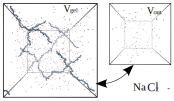
\includegraphics[width=0.7\textwidth]{figures/simgibbs}\caption{Diamond-like network in the simulation box. Color code represents
the individual ion types (red: $\na$, blue: $\cl$, yellow: $\ca$)
and the hydrogel (gray: neutral segment ($\AH$), cyan: charged segment
($\A$)). \label{fig:diamond}.}
\end{figure*}

\subsection{Model}

We model the gel as a network of 16 linear polymer chains, each by 30 monomer units. 
The chains are connected to a diamond-like polymer network throught 8 crosslinking units, and put into a simulation box with periodic boundaries (see \reffig{fig:diamond}). 
Each unit of the network carries a negative electric charge, which is equal to the charge of electron. 
Except the particles of the network, the monovalent co- and counter-ions ions, $\cl$ and $\na$, are present in simulation box. 
The total electric charge of all the particles in the box is zero, therefore the amount of $\na$ ions is bigger than that of $\cl$ by the number of hydrogel units, $\Ngel=16\cdot30 + 8=488$.

\begin{figure*}[t]
\centering 
\subfloat[Open system \label{fig: open}]
{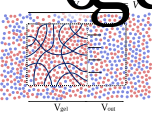
\includegraphics[width=0.5\textwidth]{figures/gc}}
\subfloat[Closed system \label{fig: closed}]
{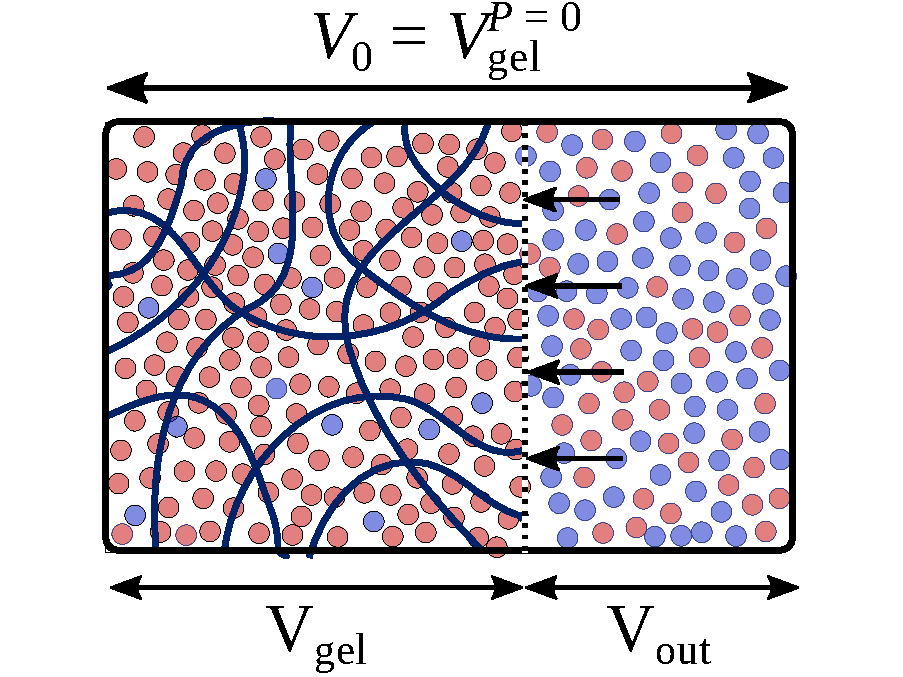
\includegraphics[width=0.5\textwidth]{figures/gibbs}}
\caption{Diamond-like network in the simulation box. Color code represents
the individual ion types (red: $\na$, blue: $\cl$, yellow: $\ca$)
and the hydrogel (gray: neutral segment ($\AH$), cyan: charged segment
($\A$)). \label{fig:open and closed}.}
\end{figure*}
We simulate the compression of the gel in two ensembles.
\begin{enumerate}
\item The first is so called \emph{open system}, when the simulation box
with gel freely exchanges ions with a big amount of aqueous solution
of certain constant salinity. 
\item And in \emph{closed system}, when the gel is in equilibrium with a
finite volume of aqueous solution.
\end{enumerate}
The compression of the gel in the \emph{open} system does not affect the surrounding salinity, thus the density of ions outside the gel remains constant $\cs =$ $\cna=$ $\ccl=$ $\text{Const}$ (\reffig{fig: open}). 
On the contrary, what remains constant in the \emph{closed} system, is the total number of $\na$ and $\cl$ ions, that are contained in the gel and in the external volume, \ie in the volume $\Vbox$ (\reffig{fig: closed}).

Let $\nna$ and $\ncl$ be the density of the corresponding ion in the compression volume, $\Vbox$ averaged over this volume
\begin{equation}
n_i = \left(N_i\gel + \cs\cdot(\Vbox - \Vgel)\right) / \Vbox
\end{equation}
where $ i \in \{\na, \cl\}$,  $N_i$ is the amount of the corresponding ions in gel.
Then in closed system $\nna$ and $\ncl$ remain constant, whereas the salinity of supernate, $\cs$, may change with the change of the gel volume.



\paragraph{Open system.}
We simulate the open system using the grand reaction method \cite{Landsgesel2020a,Rud2020}.
This method is a hybrid of molecular dynamics (MD) and Monte Carlo (MC). 
The whole simulation represents a chain of subsimulations of MD and MC followed one by each other. For MD simulation we used a standard Langevin dynamics \cite{Grest1986} which models the mechanical movement of all the system particles. 
Whereas MC simulates the thermodynamic equilibrium with reservoir, which exchanges ions with the simulation box. 
The insertion (and deletion) of ion pairs is considered as a reaction of creation (or annihilation) of an ion pair 
\[
\varnothing\stackrel{K}{\leftrightarrows}\na+\cl
\]
with a reaction constant defined by the chemical potential of ions,
$K=\exp\left(\muna+\mucl\right).$

\paragraph{Closed system.}
The similar scheme we use to simulate the gel in closed system. 
The procedure represents a chain of subsequent MD and MC simulation, but now the molecular dynamics is runing in two simulation boxes simultaneously.
The first box of the volume $\Vgel$ contains the gel with ions, and the second box, $\Vout$--- contains only ions. 
The total volume of both boxes is kept constant, $\Vbox=V_{\mathrm{gel}}+V_{\mathrm{out}}$, so the compression of the gel implies the decrease $\Vgel$ and increase $\Vout$.
These two boxes are represented in \reffig{fig:diamond}. 

\paragraph{Algorithm.}
The thermodynamic equilibrium between the two volumes implies the exchange of the ion pairs between them, which is done by means of MC procedure in a way similar to described in \cite{Panagiotopoulos1988b}.
The simulation algorithm is following:
\begin{enumerate}
\item Simulate molecular dynamics in both boxes; collect the observables, for examples, values of pressure $P$, to an array; 
\item Perform Monte-Carlo procedure simulating ion pair exchange; collect the arrays of observables samples: number of ions in both boxes, $\nna\gel$,
$\ncl\gel$, $\nna\out$ and $\ncl\out$ ; 
\item Repeat the procedure until the desired length of sample arrays is reached.
\end{enumerate}

\section{Results and discussion }

\paragraph{Compression in open system.}
\begin{figure*}[t]
\subfloat[The gel partial pressure vs gel molar volume \label{fig: PV}]
{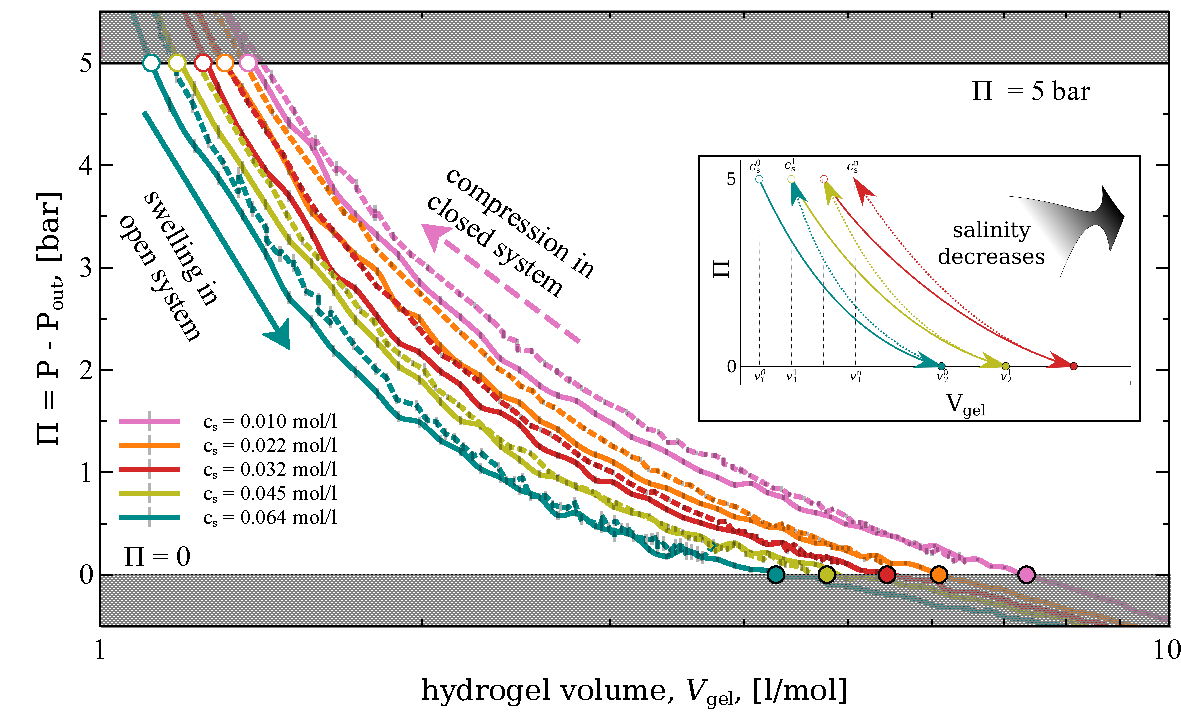
\includegraphics[width=0.48\textwidth]{figures/fig_PV_pub}}
\hspace{0.02\textwidth}
\subfloat[Supernate salinity vs gel molar volume\label{fig: CV}]
{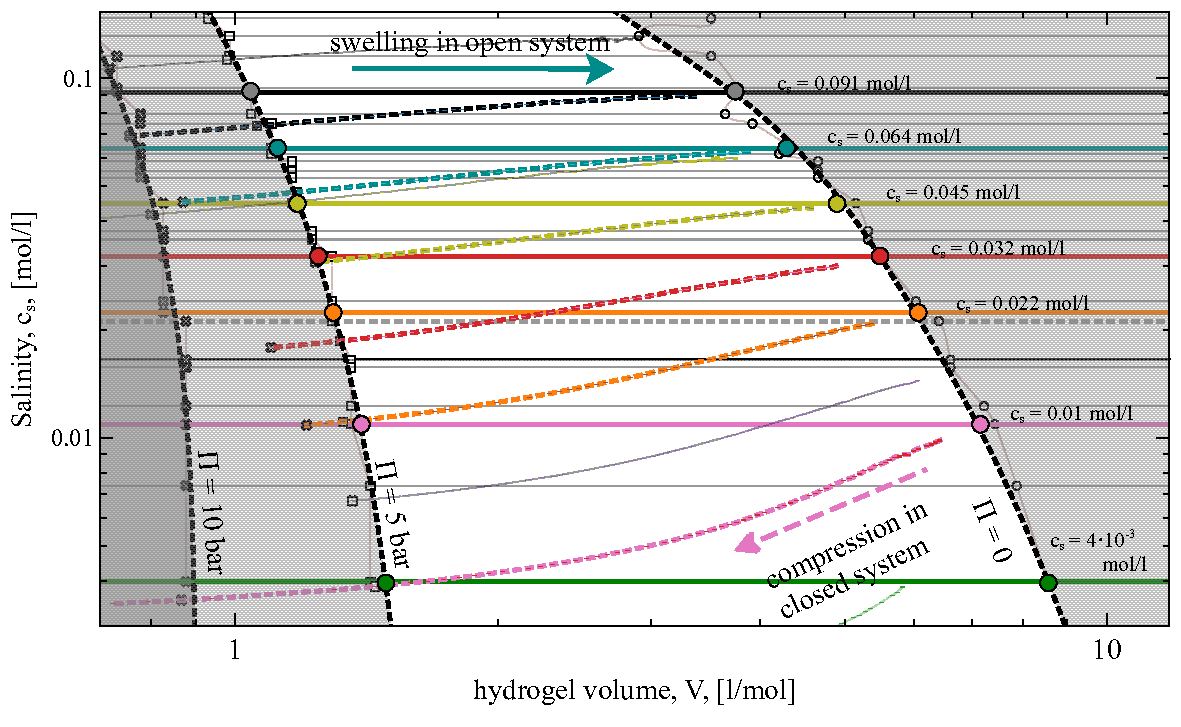
\includegraphics[width=0.48\textwidth]{figures/fig_CV_pub}}
\caption{
The compression of the gel in open system (solid lines) and in closed system (dotted lines). 
Each solid curve corresponds to different salinity of the reservoir $\cs$ (see legend). Shadowed area limit the states with applied pressure below zero and above 5 bar.\label{fig: PV and CV}}
\todoi{replace $V$ by $\Vgel$ in Figures}
\end{figure*}
First, we run a set of simulations modeling the gel compression in \emph{open system}, \ie in equilibrium with a big bath of certain salinity, $\cs$. 
The simulations are run for a set of different simulation box volumes. 
Each simulation returns the averaged pressure, $P$, and the number of $\cl$ ions, which are present in the simulation box, $\ncl$. 

In order to get the partial pressure of the gel, we substitute from $P$ the osmotic pressure of ions in the reservoir: $\Pgel=P - \Pout$.
$\Pout$, in turn, we calculate by running a separate simulation of a reservoir, containing ionic gas in equilibrium with the bath of the same salinity $\cs$. 
The gel partial pressure, $\Pgel$, is the pressure that needs to be applied to the gel via a solvent permeable filter to compress the gel to a molar-specific volume, $\Vgel$. 

The dependencies of $\Pgel$ on the gel molar volume $\Vgel$ are present in Figure \ref{fig: PV} for a set of different salinities. 
These dependencies (the case of \emph{open system}) are represented by solid lines. 
For example, the blue solid line illustrates the compression (or swelling) of the gel in equilibrium with a reservoir of salinity, $\cs=0.063$ mol/l. 
The points where the pressure equals zero, $\Pgel=0$, (indicated by filled circles) are the gel \emph{free swelling equilibrium} states. 
These states shift towards smaller volumes with increase of salinity. 
It is seen, that the increase of salinity shifts the free swelling equilibrium towards smaller volumes. 
In general, the increase of salinity shift all the $\Pgel(V)$ curves towards smaller volumes

This effect is well known and is typical for all branched \emph{strong} polyelectrolytes. 
It is caused by the decrease of ions osmotic pressure and by a screening of electrostatic interactions \cite{Zhulina2000, Landsgesel2020a}.\footnote{The salinity dependence of the size of \emph{weak} polyelectrolyte gel is in general non-monotonic. We discuss this case in \cite{Rud2018}. } %

\begin{figure*}[t]
\subfloat[Pressure vs gel molar volume \label{fig: NV}]
{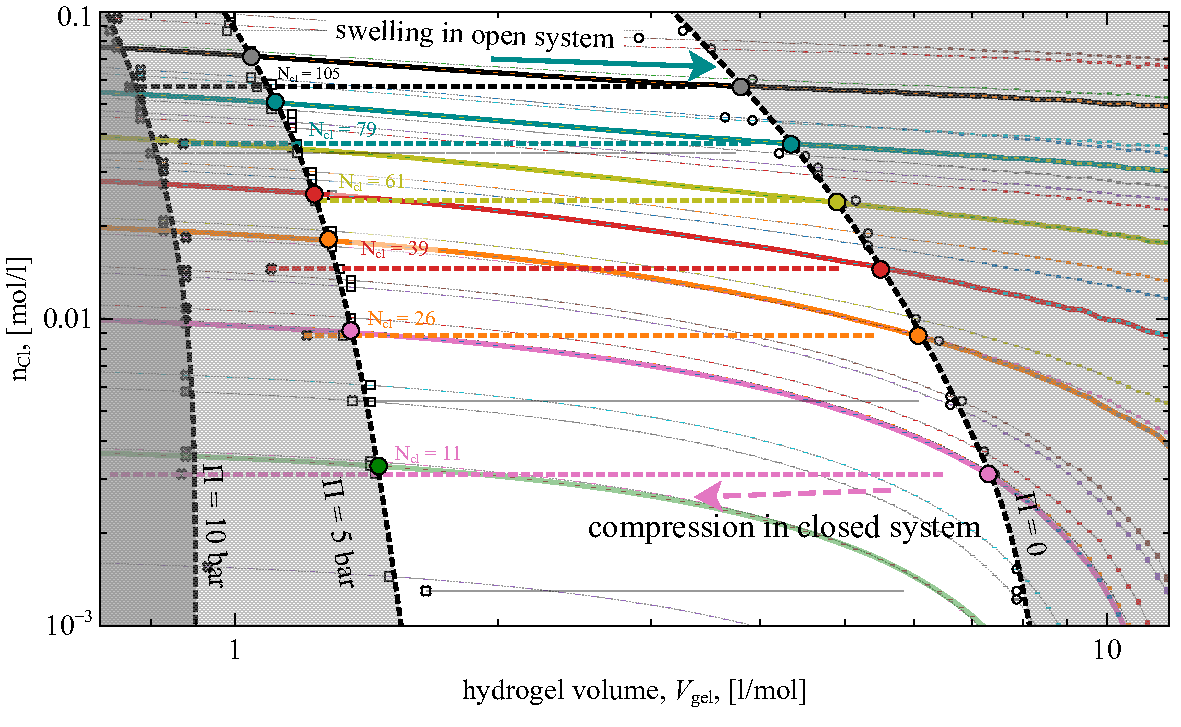
\includegraphics[width=0.49\textwidth]{figures/fig_NV_pub}}
\subfloat[Salinity vs gel molar volume\label{fig: CN}]
{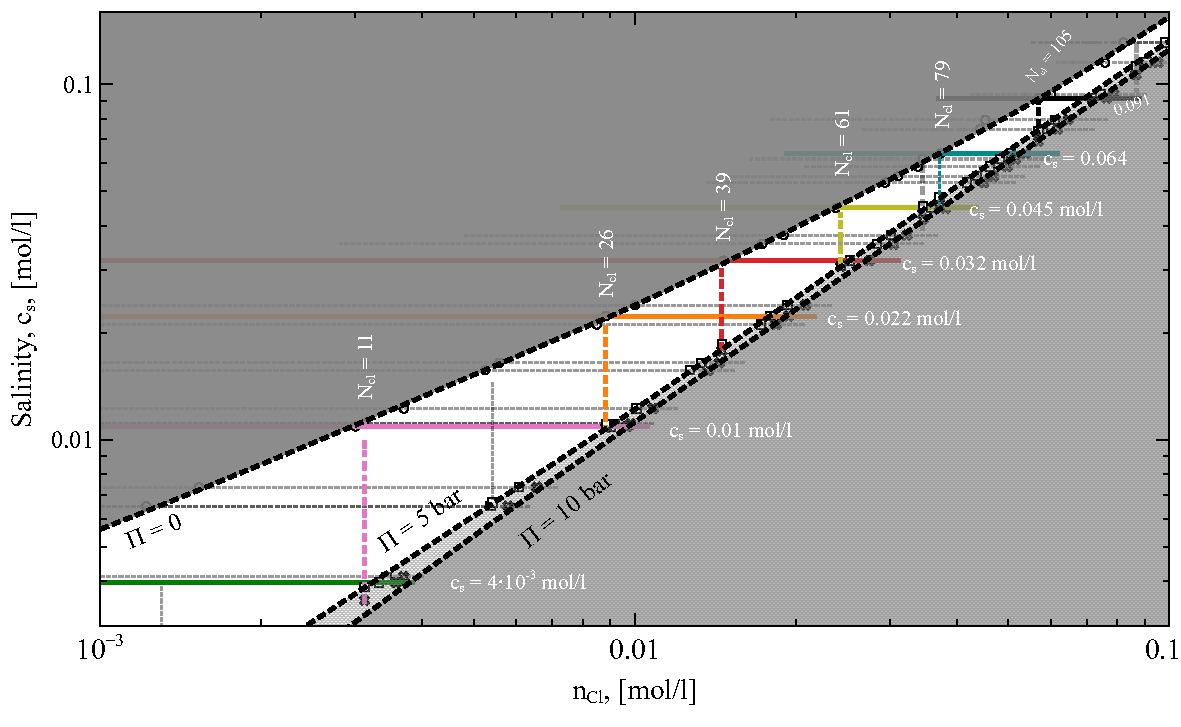
\includegraphics[width=0.495\textwidth]{figures/fig_NVbox_mu_pub}}
\caption{The compression of the gel in open system (solid lines) and in closed
system (dotted lines). Each solid curve corresponds to different salinity
of the reservoir $\cs$ (see legend). Shadowed area limit the states
with applied pressure below zero and above 5 bar.\label{fig: NV and CN}}
%\todoi{Replace y-axis labels by $\ncl$}
\end{figure*}

\paragraph{Compression in closed system.}
Each set of simulations in an \emph{open system} defines the free swelling equilibrium states of the gel for each salinity, that is the state where the gel partial pressure equals zero. 
These states are characterized by the corresponding molar volume of the gel, $\Vgel^0$ and the densities of ions in gel \{$\nna^0$, $\ncl^0$\} 
(Index ``0'' stands for zero bar applied pressure).
We use the free swelling equilibrium states as the starting ones for the gel compression in \emph{closed system}. 
Thus, we simulate the compression of the gel in the closed volume, $\Vbox$, which is equal to $\Vgel^0$, and contains $\ncl^0$ of $\cl$ ions and the $\na$ ions in the amount neutralizing the system,$\ncl^0$.

We prepare two systems, one~--- simulating the gel of the volume $\Vgel$, and another~--- simulating the supernatant solution of the volume $\Vout = \Vbox - \Vgel$.
Also, the ions of the amount $\Ncl^0$ and $\Nna^0$ are shared between the two volumes. 

The process of the gel compression in the \emph{closed} system is depicted in Figure~\ref{fig: PV} (dotted lines) as the dependence of gel partial pressure versus the gel molar volume.
In this plot, the blue dotted line, for example, illustrates the compression of the gel equilibrated with the solution of salinity $\cs=0.063$ mol/l, in a volume which gel has at zero pressure. 
Since, in this case, the volumes of the gel $\Vgel$ and of the supernate $\Vout$ are comparable, the compression of the gel affects the salinity of supernate, $\cs$. 
The supernate salinity now decreases, changing from $\cs^{0}=0.063$ at the free swelling equilibrium state to $\cs^{5}=0.045$ mol/l in the state with applied pressure $P\gel=5$ bar (index ``5'' stands for 5 bar). 

The \reffig{fig: CV} illustrates the same swelling/compression processes, but in different coordinates: \ie salinity of supernate versus the gel molar volume, $\cs(\Vgel)$.
In these coordinates, all the open system compressions show up as horizontal lines, which reflects the constant salinity, whereas the compressions in the closed system demonstrate the decrease of $\cs$.

Although the salinity during compression in \emph{open} system remains constant, the number of ions in a compression volume, i.e. in the volume where the gel is compressed (or swells), changes.
As the compression volume $\Vbox$ we chose the volume of the free swelling equilibrium state of the gel, $\Vbox = \Vgel^0$.
In the Figure \ref{fig: NV} we depicted the number of $\cl$ ions in the volume $\Vbox$, calculated per unit volume, $\ncl =$ $\Ncl/\Vbox$, as a function of the gel molar volume. 
The depicted value can be considered as the density of $\cl$ ions averaged out over the volume $\Vbox$. 

As it is expected in case of closed system these dependencies look like horizontal lines, whereas in open system, the amount of ions in compression volume increases with compression. 
This implies, that the compression of the gel in open system pulls out the ions from the bath to the compression volume, $\Vbox$. 
And vice versa, the swelling of the gel pushes ions out to the bath.

Finally, in Figure \ref{fig: CN} the same processes are depicted in coordinates $\ncl$ --- $\cs$. 
In these coordinates, both ways of the compression, in \emph{open} and in \emph{closed} system, appear as straight vertical and horizontal lines correspondingly. 


In our study, we modeled the compression of the gel in equilibrium with reservoirs of 40 different salinities, ranging from 0.001 to 0.5 mol/l. 
Every open system compression resulted in a defined free swelling equilibrium state, which we used as the initial ones for the compression in closed systems. 
All the corresponding dependencies are depicted in Figures~\ref{fig: PV and CV} and \ref{fig: NV and CN} as thin grey dashed lines (some of them are highlighted and colored).
The states corresponding to $P^{gel}=0$, 5 and 10 bar pressure are marked by open circles, squares, and crosses respectively. 
The non-shadowed areas in the Figures highlight the states in which the gel partial pressure ranges between 0 and 5 bar.

\paragraph{Desalination scheme.}
As we have seen, the compression of the gel in a closed system affects the salinity, whereas the compression in an open system affects the amount of ions in a volume where the gel is compressed in. 
Here we show how to employ these phenomena for water desalination. 
The highlighted colored lines on plots of Figures \ref{fig: PV and CV} and \ref{fig: NV and CN} form a sequence of the following one by each other swellings and compressions of the hydrogel, correspondingly in \emph{open} and \emph{closed} systems. 
This sequence forms the water desalination process.
Starting from swelling the gel in the \emph{open} system at high salinity ($\cs=0.091$ mol/l, solid black line), the gel gets compressed in \emph{closed} system until the pressure reaches 5 bar (dashed black line). 
Then the same gel swells in a reservoir of a bit lower salinity (\ie $\cs=0.064$ mol/l, light blue line). 
After swelling, the gel is compressed again by the pressure of 5 bar in \emph{closed} system (dashed light blue line).  
Then it is put swelling in a reservoir of even smaller salinity ($\cs=0.045$ mol/l, solid yellow line). 
And so on. 
The chain of alternating swelling and compression steps ends up when salinity gets equal to $\cs=4\cdot10^{-3}$ mol/l after compression in closed system (dashed magenta line).

The plots of Figures \ref{fig: PV and CV} and \ref{fig: NV and CN} depict the whole process in all the possible coordinates
In all the plots the whole process looks like a staircase, especially in the Figure~\ref{fig: CN}, where open system processes are horizontal lines and closed system are vertical ones, a 'staircase' has rectangular steps

%\begin{enumerate}
%    \item as gel partial pressure versus gel molar volume, $\Pgel(\Vgel)$ (\ref{fig: PV}), 
%    \item as supernatant salinity versus gel molar volume, $\cs(\Vgel)$ (\ref{fig: CV}),
%    \item the amount of $\cl$ ions in a compression volume versus gel volume, $\ncl(\Vgel)$ (\ref{fig: NV}), 
%    \item $\ncl$ as function of supernatant salinity.
%\end{enumerate}


\todo{we could get rid of saying 'gel molar volume' if we state elsewhere that all the values are calculated per one mol of the gel}

%Then we repeat the simulation of hydrogel swelling in open system but setting as a salinity of the reservoir the new, obtained from the previous process, value $\cs=$ 0.045 mol/l. 
%Again, as soon as we obtain the free swelling equilibrium state (at new salinity), with corresponding new values of $V\gel$ and $\ncl$, we start simulating the compression in closed system. Now the salinity changes again, decreasing from 0.045 to 0.031 mol/l (at 5 bar). 
%These two processes are depicted by solid and dotted yellow lines in Figure~\ref{fig:fig_PV}.
%The Figure shows also the repetition of this procedure three more times until the salinity reaches the value $\cs=0.01$ mol/l. 
%The last dashed magenta line shows the compression in closed system which ends up with $\cs=4\cdot10^{-4}$ mol/l. 
%Schematically this process is depicted in the inset to the plot.



%The same process is depicted on Figure~\ref{fig:fig_CV} but in different coordinates: salinity versus volume. 
%In this coordinates the swelling in open system appear to be horizontal line, since the salinity in this process is constant. 
%Again we start from swelling in open system untill the gel reaches its free swelling equilibrium (solid blue line).
%Then the gel is compressed in closed system (dashed blue line), ending up in a state with applied to the gel pressure 5 bar. 
%In this process the surrounding solution salinitiy changes from 0.064 to 0.045 mol/l.
%Then the gel again swells in open system, but at new salinity. 

\paragraph{The efficiency of desalination.}
The theoretical minimum specific energy for seawater desalination ($\cs=35$ g/l, $\simeq0.6$ mol/l as for pure NaCl) is 1.1 kWh/m3 (3.9 kJ/L) for 50\% recovery \cite{Wang_2020}.
This value is calculated as follows 
\begin{equation}
W=2RT\left(\frac{c_{f}}{R_{w}}\ln\frac{c_{b}}{c_{f}}-c_{p}\ln\frac{c_{b}}{c_{p}}\right)
\label{eq:SEC}
\end{equation}
where $R$ is a universal gas constant, $c_{f}$ is the salinity of feed water, $c_p$~--- of product water and $c_b$~--- the salinity of the brine, which necessarily appears in any desalination process. 
$R_{w}$ is a recovery ratio, \ie the ratio between volume of produced water and the volume of the feed water. 
50\% recovery ratio means that one part of feed water divides into two equal volume solutions of the product water and of the brine.
Of course, a significant amount of additional energy is required to operate the system\cite{Kim_2019}. 
It has been reported that the specific energy consumption (SEC) of reverse osmosis (RO) process is 2.5~-- 4.0 kWh/m3 (9~-- 14.4 kJ/l), which is significantly higher than its minimum specific energy.
The SEC of a real-scale RO plant is even higher, approximately 3.5~-- 4.5 kWh/$m^{3}$ (12.6 - 16.2 kJ/L), including pre-treatment and post-treatment processes \cite{Kim_2018}. 
%Because of the inherent high energy requirement for RO desalination, seawater is not commonly utilized over traditional surface water.



In order to compare the efficiency of the process presented in \ref{fig: PV and CV} and \ref{fig: NV and CN} with provided values we collect the corresponding data to the Table~\ref{tab: table}.
The presented desalination process is a cascade of six swellings in open system, at six different (constant) salinities $\cs$, each followed by six compressions in closed system, at six different (constant) $\ncl$.
Each swelling and compression presented as a row of the Table~\ref{tab: table}, which is collored to matching to the lines on Figures.
The first column of the table contains values $\cs^0$ and $\cs^5$, which stand for the supernatant salinity at 0 and 5 bar compression; in open system supernatant salinity does not change, so $\cs^0$ and $\cs^5$ are presented by a single number. 
The second column contains values of $n^0$ and $n^5$, which stand for the number of $\cl$ ions in compression volume at 0 and 5 bar pressure. \todo[fancyline]{it is not a number but a number in unit volume}
The number of ion does not change in closed system compression, thus $n^0$ and $n^5$ are the same in corresponding row.
The fourth column shows the change of the volume in corresponding process, $\Delta v$. 
The fifth column contain the work needed for the compression in the corresponding process, calculated per volume of extracted solution. 
This value is calculated as integral of corresponding $\Pgel(\Vgel)$ dependence
\begin{equation}
    W = \frac{\int_{v^0}^{v^5} \Pgel d\Vgel}{\Delta v}
\end{equation}
Here, in the table we present the absolute value, whereas one should keep in mind that the compression implies the work which is done by external force, whereas the swelling implies the work which is done by gel.
\todo{may be we return back the 'minuses' to the W values}

\begin{table}
\begin{tabular*}{1\textwidth}{@{\extracolsep{\fill}}ll|lc|c|l|l|ll}
\multicolumn{1}{l|}{$c_{s}^{0}$, mM} & $c_{s}^{5}$, mM & \multicolumn{1}{l|}{$n_{\cl}^{0}$, mM} & $n_{\cl}^{5}$, mM & $\Delta v$, l & $R_{w}$ & $|W$\textbar , J/L & \multicolumn{2}{c}{$W^{id}$, J/L}\tabularnewline
\hline 
\hline 
\multirow{2}{*}{{\small{}$91.47$}} & \multirow{2}{*}{} & \multicolumn{2}{l|}{{\small{}$57.08\pm0.122\enskip\longrightarrow$}} & \multirow{2}{*}{{\small{}2.74}} & \multirow{2}{*}{} & \multirow{2}{*}{{\small{}$95.4\pm1.86$}} &  & \multirow{2}{*}{}\tabularnewline
 &  & \multicolumn{2}{r|}{{\small{}$71.75\pm0.024$}} &  &  &  & \multirow{8}{*}{{\small{}\hspace{-1em}}\textcolor{teal}{\small{}$\left.\begin{array}{l}
\\
\\
\\
\\
\\
\\
\\
\end{array}\right\rbrace $$\rotatebox{90}{\hspace{-3.8em}\ensuremath{\begin{array}{cc}
W^{id}= & (52.9)\\
R_{w}= & 0.54
\end{array}}}$}} & \tabularnewline
\cline{1-7} \cline{2-7} \cline{3-7} \cline{4-7} \cline{5-7} \cline{6-7} \cline{7-7} 
\multicolumn{2}{l|}{{\small{}$89.41\pm0.229\enskip\longrightarrow$}} & \multirow{2}{*}{{\small{}56.90}} & \multirow{2}{*}{} & \multirow{2}{*}{{\small{}2.72}} & \multirow{2}{*}{} & \multirow{2}{*}{{\small{}$109.1\pm1.72$}} &  & \multirow{2}{*}{}\tabularnewline
\multicolumn{2}{r|}{{\small{}$73.63\pm0.03$}} &  &  &  &  &  &  & \tabularnewline
\cline{1-7} \cline{2-7} \cline{3-7} \cline{4-7} \cline{5-7} \cline{6-7} \cline{7-7} 
\multirow{2}{*}{\textcolor{teal}{\small{}63.93}} & \multirow{2}{*}{} & \multicolumn{2}{l|}{\textcolor{teal}{\small{}$37.28\pm0.083\enskip\longrightarrow$}} & \multirow{2}{*}{\textcolor{teal}{\small{}3.26}} & \multirow{2}{*}{\textcolor{teal}{\small{}0.54}} & \multirow{2}{*}{\textcolor{teal}{\small{}$100.9\pm1.69$}} &  & \tabularnewline
 &  & \multicolumn{2}{r|}{\textcolor{teal}{\small{}$50.58\pm0.013$}} &  &  &  &  & \multirow{8}{*}{{\small{}\hspace{-1em}}\textcolor{olive}{\small{}$\left.\begin{array}{l}
\\
\\
\\
\\
\\
\\
\\
\end{array}\right\rbrace $$\rotatebox{90}{\hspace{-3.8em}\ensuremath{\begin{array}{cc}
W^{id}= & 38.2\\
R_{w}= & 0.53
\end{array}}}$}}\tabularnewline
\cline{1-7} \cline{2-7} \cline{3-7} \cline{4-7} \cline{5-7} \cline{6-7} \cline{7-7} 
\multicolumn{2}{l|}{\textcolor{teal}{\small{}$62.05\pm0.15\enskip\longrightarrow$}} & \multirow{2}{*}{\textcolor{teal}{\small{}37.17}} & \multirow{2}{*}{} & \multirow{2}{*}{\textcolor{teal}{\small{}3.18}} & \multirow{2}{*}{} & \multirow{2}{*}{\textcolor{teal}{\small{}$107.4\pm1.37$}} &  & \tabularnewline
\multicolumn{2}{r|}{\textcolor{teal}{\small{}$48.21\pm0.016$}} &  &  &  &  &  &  & \tabularnewline
\cline{1-7} \cline{2-7} \cline{3-7} \cline{4-7} \cline{5-7} \cline{6-7} \cline{7-7} 
\multirow{2}{*}{\textcolor{olive}{\small{}44.91}} & \multirow{2}{*}{} & \multicolumn{2}{l|}{\textcolor{olive}{\small{}$23.75\pm0.057\enskip\longrightarrow$}} & \multirow{2}{*}{\textcolor{olive}{\small{}3.82}} & \multirow{2}{*}{\textcolor{olive}{\small{}0.53}} & \multirow{2}{*}{\textcolor{olive}{\small{}$106.7\pm1.51$}} &  & \tabularnewline
 &  & \multicolumn{2}{r|}{\textcolor{olive}{\small{}$35.91\pm0.010$}} &  &  &  & \multirow{8}{*}{{\small{}\hspace{-1em}}\textcolor{red}{\small{}$\left.\begin{array}{l}
\\
\\
\\
\\
\\
\\
\\
\end{array}\right\rbrace \rotatebox{90}{\hspace{-3.8em}\ensuremath{\begin{array}{cc}
W^{id}= & 43.8\ {\color{red}{\scriptstyle (41.0)}}\\
R_{w}= & 0.52\ {\scriptstyle (0.46)}
\end{array}}}$}} & \tabularnewline
\cline{1-7} \cline{2-7} \cline{3-7} \cline{4-7} \cline{5-7} \cline{6-7} \cline{7-7} 
\multicolumn{2}{l|}{\textcolor{olive}{\small{}$43.46\pm0.12\enskip\longrightarrow$}} & \multirow{2}{*}{\textcolor{olive}{\small{}24.27}} & \multirow{2}{*}{} & \multirow{2}{*}{\textcolor{olive}{\small{}3.91}} & \multirow{2}{*}{} & \multirow{2}{*}{\textcolor{olive}{\small{}$106.4\pm1.13$}} &  & \tabularnewline
\multicolumn{2}{r|}{\textcolor{olive}{\small{}$30.80\pm0.008$}} &  &  &  &  &  &  & \tabularnewline
\cline{1-7} \cline{2-7} \cline{3-7} \cline{4-7} \cline{5-7} \cline{6-7} \cline{7-7} 
\multirow{2}{*}{\textcolor{red}{\small{}31.93}} & \multirow{2}{*}{} & \multicolumn{2}{l|}{\textcolor{red}{\small{}$14.66\pm0.037\enskip\longrightarrow$}} & \multirow{2}{*}{\textcolor{red}{\small{}4.20}} & \multirow{2}{*}{\textcolor{red}{\small{}0.52}} & \multirow{2}{*}{\textcolor{red}{\small{}$107.9\pm1.42$}} &  & \tabularnewline
 &  & \multicolumn{2}{r|}{\textcolor{red}{\small{}$25.30\pm0.006$}} &  &  &  &  & \multirow{8}{*}{{\small{}\hspace{-1em}}\textcolor{orange}{\small{}$\left.\begin{array}{l}
\\
\\
\\
\\
\\
\\
\\
\end{array}\right\rbrace \rotatebox{90}{\hspace{-3.8em}\ensuremath{\begin{array}{cc}
W^{id}= & 66.6\ {\scriptstyle (22.0)}\\
R_{w}= & 0.53\ {\scriptstyle (0.49)}
\end{array}}}$}}\tabularnewline
\cline{1-7} \cline{2-7} \cline{3-7} \cline{4-7} \cline{5-7} \cline{6-7} \cline{7-7} 
\multicolumn{2}{l|}{\textcolor{red}{\small{}$30.03\pm0.084\enskip\longrightarrow$}} & \multirow{2}{*}{\textcolor{red}{\small{}14.55}} & \multirow{2}{*}{} & \multirow{2}{*}{\textcolor{red}{\small{}$\begin{array}{c}
4.17\\
{\scriptstyle (3.22)}
\end{array}$}} & \multirow{2}{*}{} & \multirow{2}{*}{\textcolor{red}{\small{}$\begin{array}{c}
115.6\pm0.92\\
{\scriptstyle (57.3)}
\end{array}$}} &  & \tabularnewline
\multicolumn{2}{r|}{\textcolor{red}{\small{}$\begin{array}{c}
18.59\pm0.004\,\\
{\scriptstyle (22.32)}
\end{array}$}} &  &  &  &  &  &  & \tabularnewline
\cline{1-7} \cline{2-7} \cline{3-7} \cline{4-7} \cline{5-7} \cline{6-7} \cline{7-7} 
\multirow{2}{*}{\textcolor{orange}{\small{}22.30}} & \multirow{2}{*}{} & \multicolumn{2}{l|}{\textcolor{orange}{\small{}$8.84\pm0.026\enskip\longrightarrow$}} & \multirow{2}{*}{\textcolor{orange}{\small{}$\begin{array}{c}
4.75\\
{\scriptstyle (3.76)}
\end{array}$}} & \multirow{2}{*}{\textcolor{orange}{\small{}0.53}} & \multirow{2}{*}{\textcolor{orange}{\small{}$\begin{array}{c}
108.1\pm1.26\\
{\scriptstyle (68.3)}
\end{array}$}} &  & \tabularnewline
 &  & \multicolumn{2}{r|}{\textcolor{orange}{\small{}$\begin{array}{c}
\text{17.95}\pm\text{0.004}\\
{\scriptstyle (14.56)}
\end{array}$}} &  &  &  & \multirow{7}{*}{{\small{}\hspace{-1em}}\textcolor{magenta}{\small{}$\left.\begin{array}{l}
\\
\\
\\
\\
\\
\\
\end{array}\right\rbrace \rotatebox{90}{\hspace{-3em}\ensuremath{\begin{array}{cc}
W^{id}= & 69.7\\
R_{w}= & 0.55
\end{array}}}$}} & \tabularnewline
\cline{1-7} \cline{2-7} \cline{3-7} \cline{4-7} \cline{5-7} \cline{6-7} \cline{7-7} 
\multicolumn{2}{l|}{\textcolor{orange}{\small{}$20.74\pm0.064\enskip\longrightarrow$}} & \multirow{2}{*}{\textcolor{orange}{\small{}8.83}} & \multirow{2}{*}{} & \multirow{2}{*}{\textcolor{orange}{\small{}$4.71$}} & \multirow{2}{*}{} & \multirow{2}{*}{\textcolor{orange}{\small{}$110.8\pm0.77$}} &  & \tabularnewline
\multicolumn{2}{r|}{\textcolor{orange}{\small{}$11.08\pm0.002$}} &  &  &  &  &  &  & \tabularnewline
\cline{1-7} \cline{2-7} \cline{3-7} \cline{4-7} \cline{5-7} \cline{6-7} \cline{7-7} 
\multirow{2}{*}{\textcolor{magenta}{\small{}10.90}} & \multirow{2}{*}{} & \multicolumn{2}{l|}{\textcolor{magenta}{\small{}$3.00\pm0.01\enskip\longrightarrow$}} & \multirow{2}{*}{\textcolor{magenta}{\small{}6.08}} & \multirow{2}{*}{\textcolor{magenta}{\small{}0.55}} & \multirow{2}{*}{\textcolor{magenta}{\small{}$106.9\pm1.05$}} &  & \tabularnewline
 &  & \multicolumn{2}{r|}{\textcolor{magenta}{\small{}9.01$\pm$0.002}} &  &  &  &  & \tabularnewline
\cline{1-7} \cline{2-7} \cline{3-7} \cline{4-7} \cline{5-7} \cline{6-7} \cline{7-7} 
\multicolumn{2}{l|}{\textcolor{magenta}{\small{}$9.83\pm0.046\enskip\longrightarrow$}} & \multirow{2}{*}{\textcolor{magenta}{\small{}3.12}} & \multirow{2}{*}{} & \multirow{2}{*}{\textcolor{magenta}{\small{}5.78}} & \multirow{2}{*}{} & \multirow{2}{*}{\textcolor{magenta}{\small{}$119.4\pm0.97$}} &  & \tabularnewline
\multicolumn{2}{r|}{\textcolor{magenta}{\small{}$3.86\pm0.001$}} &  &  &  &  &  &  & \tabularnewline
\end{tabular*}

\caption{All the units calculated per one mol of gel segments. Values in brackets
are the estimates corresponding to crossection of 'red' and 'orange'
lines on the plots of figures \ref{fig: PV and CV} and \ref{fig: NV and CN}
}
\end{table}





The fifth column \todo{check if it is fifth column} contains the values of specific energy consumption, $W^\text{id}$, which are calculated as follows.
We consider, for example, the solution of concentration $\cs^f=0.045$ mol/l as a feed solution, and the solutions of $\cs^p=0.032M$ and $\cs^b = 0.064$ mol/l 
correspondingly as produced product and brine solutions.
\begin{enumerate}
    \item first, the gel, equilibrated with feed solution, is getting compressed in a closed system.
    while compression it changes its volume by $\Delta v^p = 3.69$  l/mol and the salinity of supernate decreases from $\cs^f$ to $\cs^p$.
    The volume of product solution equals to $\Delta v^p$
    \item Then the squeezed gel is put back to feed solution and is getting equilibrated there under pressure, so it does not swell. 
    \item then the squeezed gel is let to swell in closed system such that the salinity of external solution increases reaching the value of $\cs^b$
    \item finally, the gel is taken out and squeezed by 5 bar in open system in equilibrium with the bath of the brine. 
    The change of the gel volume in this process is $\Delta v^b = 3.26$ l/mol, which equals to the volume of produced brine. 
\end{enumerate}
Thus the recovery ratio $R_w = \Delta v^p / (\Delta v^p + \Delta v^b) \simeq $ 0.53 and the theoretical minimum specific energy of desalination with corresponding $\cs^f$, $\cs^p$ and $\cs^b$ is $W^{id} =$ 38.2 J/l (\refeq{eq:SEC})




\todoi{Start from here next time}


\section{Conclusions}
\begin{enumerate}
\item We have modeled the compression of the gel in thermodynamic equilibrium
with the reservoir of limited amount of water.
\item We have shown that in case of gel made of strong polyelectrolyte,
the compression always lead to decrease of the surrounding salinity.
\item We have modeled the process of water desalination combining two processes:
(1) the swelling of the gel in open system, exchanging ions with big
reservoir at constant salinity. (2) the compression of the gel in
closed system, when the gel affect the salinity in surrounding solution.
\item We estimated the energy needed to produce one liter of water and have
show that the method at least theoretically may compete with the modern
technologies used in industry nowadays.
\end{enumerate}

\section*{Acknowledgments}

This research was supported by the Czech Science Foundation (grant
19-17847Y) (OR, LN, AK), Government of Russian Federation, grant number
14.W03.31.0022. AK thanks the Grant Agency of Charles University for
support (project 318120). Computational resources were supplied by
the project ``e-Infrastruktura CZ'' (e-INFRA LM2018140) provided
within the program Projects of Large Research, Development and Innovations
Infrastructures.

\bibliography{lit/gibbs}

\newpage
\listoftodos

\newpage
\section*{Supplementary Information}
\subsection{Sampling routine}
Data gained from Molecular Dynamics (MD) and Markov Chain Monte Carlo processes (MD) are highly autocorrelated, thus we can not imply statistic developed for uncorrelated data. We have written a small in-house python package to calculate the expected value, the margin of error and effective sample size of correlated data.

The goal of the routine is to estimate mean and margins of error for an observable e.g. pressure, number of particles, end-to-end distance of a chain for a given confidence level or effective sample size. 

We also provided the way to limit sampling procedure with some timeout value. Our routine based on [] %[https://www.physik.uni-leipzig.de/~janke/Paper/nic10_423_2002.pdf]

There are multiple sampling routines developed for autocorrelated data, i.e. binning analysis, ... %some notes what others do

Expected value of the observable $X$ estimated as the mere mean of the sample $\overline{X}$, the same way one would do for uncorrelated data, whilst to estimate margins of error and \emph{effective} sample size $N_{eff}$ we used the next formulae. 
First of all we have to correct sample size to account that data is correlated:
\begin{eqnarray}
    N_{eff} = \frac{N}{2\tau}
    \\
    \tau  = \frac{1}{2} + \sum_{k=1}^{N} \text{acf} (k) (1-\frac{k}{N})
\end{eqnarray}
where $\tau$ is integrated autocorrelation time, $N$ size of autocorrelated data, $\text{acf} (k)$ is autocorrelation function on lag.

Note that ideally integral of  $\text{acf} (k)$ monotonically approaches some finite value, but due to unavoidable errors in number representation in computer and numeric integration methods it does not hold. 
For that reason instead of $\text{acf} (k)$ integral we use the maximum of its cumulative sum.

Margins of error (MOE) for a given confidence level $\gamma$ and effective sample size $N_{eff}$ is calculated using the next equation:
\begin{eqnarray}
    \text{MOE}(\gamma) = \frac{S_{N}}{\sqrt{N_{eff}}} t_{((1+\gamma)/2, N_{eff}-1)}
\end{eqnarray}
where $t_{(\alpha, \nu)}$ is percentile function (inverse cumulative distribution function) of Student’s distribution with $\nu$ degrees of freedom for $\alpha$ percentile,
$S_N$ is standard deviation of the sample.

The true mean of the observable $\mu_X$ lies inside the confidence interval with the confidence level $\gamma$.
\begin{equation}
    \Pr(\overline{X} - MOE(\gamma) \leq \mu_X \leq \overline{X} + MOE(\gamma)) = \gamma
\end{equation}

In our study we set $\gamma = 0.95$


\subsubsection{Routine implementation details}
%Probably we don't need this section

The arguments of our sampling routine are a function to calculate next sample and one of the next arguments: margins of error, effective sample size and timeout.

An observable is sampled in a loop till one of required targets is met (timeout, the margins of error or sample size). 
In the each following iteration of the loop, mean value and the margins of error are calculated with ever increasing precision and sample size. 

The loop follows the next steps:
\begin{itemize}
    \item Sample new data to double the sample size
    \item Recalculate $\tau$, $N_{eff}$, MOE
    \item If MOE is less, or $N_{eff}$ is bigger than desired, or run time exceed timeout exit loop
\end{itemize}

The routine returns mean of the sample, margins of error that defines confidence interval where true mean of distribution lies and \emph{effective} sample size that accounts that data is autocorrelated.

The routine is also described in Figure \ref{fig: sampling_diagram}

\begin{figure*}[t]
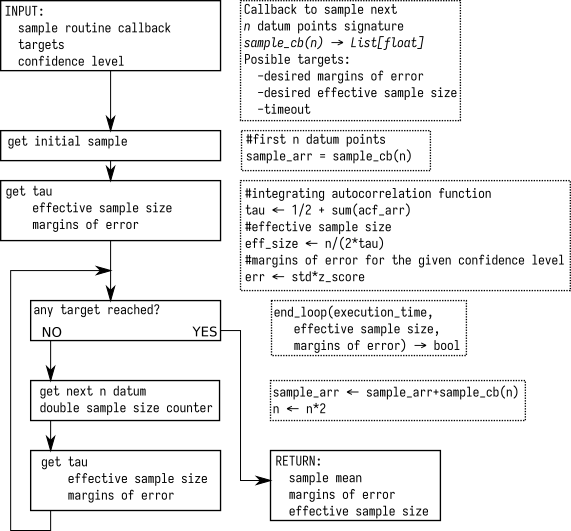
\includegraphics[width = 0.9\textwidth]{figures/sample_to_target_scheme.png}
\caption{Sampling routine diagram}
\label{fig: sampling_diagram}
\end{figure*}

\subsection{Monte Carlo process}
\subsubsection{Open system}
Free energy in grand-cannonical ensemble
\begin{equation}
\Omega = E-TS + \mu N 
\end{equation}
where $S$ is the entropy. Boltzman formula
\begin{equation}
S= k_B \ln \frac{V^N}{N!}
\end{equation}
The change of free energy associated with insertion ($\xi=1$) or deletion ($\xi=-1$) a particle is
\begin{equation}
\Delta \Omega =\kT\ln\left(V^{\xi}\frac{N!}{ (N+\xi)!}\right)+\xi\mu+\Delta E
\end{equation}
\subsubsection{Closed system}
In closed system ion pairs are exchanged between two finite volume boxes.

\begin{equation}
    \na_{I} + \cl_{I} \leftrightarrows \na_{II} + \cl_{II}
\end{equation}

Suppose an ion pair has been moved from box to another, then the change in entropy can be expressed as
\begin{eqnarray}
    \Delta S = 2 \log \left(\frac{V^{I}}{V^{II}} \right) ^ {\gamma}  \left(\frac{(N_{Na^{+}}^{I}+\mathcal{H}(\gamma))(N_{Cl^{-}}^{I}+\mathcal{H}(\gamma))}{(N_{Na^{+}}^{II}+\mathcal{H}(-\gamma))(N_{Cl^{-}}^{II}+\mathcal{H}(-\gamma))}\right)^{-\gamma}
\end{eqnarray}
where $\gamma$ defines the direction of the trial move, so that $\gamma_{I \rightarrow II} = -1$ when an ion pair moved from box I to box II and  $\gamma_{II \rightarrow I} = 1$ otherwise, $\mathcal{H}$ is the Heaviside step function.

The probability that the move will be accepted is calculated from the free energy change as
\begin{equation}
    \mathcal{P} = \exp(-\beta (\Delta E_{pot} - k_B T \Delta S))
\end{equation}

Thus, moving an ion pair from box I to box II change the entropy
\begin{equation}
    \Delta S_{I \rightarrow II} = 2 \log \left(\frac{V^{II}}{V^{I}} \right)  \frac{N_{Na^{+}}^{I} N_{Cl^{-}}^{I}}{(N_{Na^{+}}^{II}+1)(N_{Cl^{-}}^{II}+1)}
\end{equation}

The probability of this move ${I \rightarrow II}$ to be accepted

\begin{equation}
    \mathcal{P}_{I \rightarrow II} = \exp\left(-\beta (\Delta E_{pot} - 2 k_B T \log \left(\frac{V^{II}}{V^{I}} \right)  \frac{N_{Na^{+}}^{I} N_{Cl^{-}}^{I}}{(N_{Na^{+}}^{II}+1)(N_{Cl^{-}}^{II}+1)})\right)
\end{equation}

\begin{itemize}
\item perform a move of a random ion pair 
    \begin{equation}
    \left(\na +\cl\right)^{I} \leftrightarrows\left(\na +\cl\right)^{II}
\end{equation}

\item accept if 
    \begin{equation}
    \mathrm{rand}(0,1] < \left(\frac{V^{II}}{V^{I}}\right)^{\xi}\prod_{i=Na,\ Cl}\frac{N^I_i!}{(N^I_i+\xi)!}\frac{N^{II}_i!}{(N^{II}_i+\xi)!}\exp(-\beta\Delta E_{pot})
\end{equation}
\end{itemize}


\subsection{Donnan equilibrium in finite volume reservoirs}
Before we can explore any system properties and collect data the system has to be equilibrated. To achieve this we perform equilibration routine consist of sequence of Molecular Dynamics and Monte Carlo steps.
%Here we describe our technique
The result of equilibration is stationary of any observable such as pressure, end-to-end distance for polymer chains and ion distribution between reservoirs. 

The success and the cost in terms of computational time for the equilibration process heavily depend on initial guess. In our case we initialize the system with ion distribution corresponds to Donnan equilibrium.

In closed system number of ions in the system is constant, so Donnan equilibrium can be formulated as follows
\begin{equation}
    \frac{\left(N_{pairs} - N_{Cl^{-}}^{(gel)}\right)^2}{V_{salt}^2} = \frac{N_{Cl^{-}}^{gel} (N^{{(gel)}}_{A^{-}} + N_{Cl^{-}}^{(gel)})}{V_{gel}^2}
\end{equation}
where $N^{{(gel)}}_{A^{-}}$ is number of fixed anions in the box with the gel \ie acetic groups in the polymer gel.
Solving this equation with respect to $N^{{(gel)}}_{A^{-}}$ gives us the distribution of the ions between two boxes.

%probably not needed
\begin{eqnarray}
    %N_{Cl^{-}}^{(gel)} = \frac{\frac{N^{{(gel)}}_{A^{-}} V_{salt}^{2}}{2} + N_{pairs} V_{gel}^{2} - \frac{V_{salt} \sqrt{N^{{(gel)}}_{A^{-}}^{2} V_{salt}^{2} + 4 N^{{(gel)}}_{A^{-}} N_{pairs} V_{gel}^{2} + 4 N_{pairs}^{2} V_{gel}^{2}}}{2}}{V_{gel}^{2} - V_{salt}^{2}}
    \\
    N_{Na^{+}}^{(gel)} = N^{{(gel)}}_{A^{-}} + N_{Cl^{-}}^{(gel)}
    \\
    N_{Cl^{-}}^{(salt)} = N_{Na^{+}}^{(gel)} = N_{pairs} - N_{Cl^{-}}^{(gel)}
\end{eqnarray}




\begin{table}
\begin{tabular*}{1\textwidth}{@{\extracolsep{\fill}}ll|lc|c|l|l|ll}
\multicolumn{1}{l|}{$c_{s}^{0}$, mM} & $c_{s}^{5}$, mM & \multicolumn{1}{l|}{$n_{\cl}^{0}$, mM} & $n_{\cl}^{5}$, mM & $\Delta v$, l & $R_{w}$ & $|W$\textbar , J/L & \multicolumn{2}{c}{$W^{id}$, J/L}\tabularnewline
\hline 
\hline 
\multirow{2}{*}{{\small{}91.466}} & \multirow{2}{*}{} & \multicolumn{2}{l|}{{\small{}$57.083\pm0.1215\quad\longrightarrow$}} & \multirow{2}{*}{{\small{}2.74}} & \multirow{2}{*}{} & \multirow{2}{*}{{\small{}$95.4\pm1.86$}} &  & \multirow{2}{*}{}\tabularnewline
 &  & \multicolumn{2}{r|}{{\small{}$71.751\pm0.024$}} &  &  &  & \multirow{8}{*}{{\small{}\hspace{-1em}}\textcolor{teal}{\small{}$\left.\begin{array}{l}
\\
\\
\\
\\
\\
\\
\\
\end{array}\right\rbrace $$\rotatebox{90}{\hspace{-3.8em}\ensuremath{\begin{array}{cc}
W^{id}= & (52.9)\\
R_{w}= & 0.54
\end{array}}}$}} & \tabularnewline
\cline{1-7} \cline{2-7} \cline{3-7} \cline{4-7} \cline{5-7} \cline{6-7} \cline{7-7} 
\multicolumn{2}{l|}{{\small{}$89.414\pm0.2286\quad\longrightarrow$}} & \multirow{2}{*}{{\small{}56.898}} & \multirow{2}{*}{} & \multirow{2}{*}{{\small{}2.72}} & \multirow{2}{*}{} & \multirow{2}{*}{{\small{}$109.1\pm1.72$}} &  & \multirow{2}{*}{}\tabularnewline
\multicolumn{2}{r|}{{\small{}$73.633\pm0.029$}} &  &  &  &  &  &  & \tabularnewline
\cline{1-7} \cline{2-7} \cline{3-7} \cline{4-7} \cline{5-7} \cline{6-7} \cline{7-7} 
\multirow{2}{*}{\textcolor{teal}{\small{}63.93}} & \multirow{2}{*}{} & \multicolumn{2}{l|}{\textcolor{teal}{\small{}$37.281\pm0.083\quad\longrightarrow$}} & \multirow{2}{*}{\textcolor{teal}{\small{}3.26}} & \multirow{2}{*}{\textcolor{teal}{\small{}0.54}} & \multirow{2}{*}{\textcolor{teal}{\small{}$100.9\pm1.69$}} &  & \tabularnewline
 &  & \multicolumn{2}{r|}{\textcolor{teal}{\small{}$50.579\pm0.0134$}} &  &  &  &  & \multirow{8}{*}{{\small{}\hspace{-1em}}\textcolor{olive}{\small{}$\left.\begin{array}{l}
\\
\\
\\
\\
\\
\\
\\
\end{array}\right\rbrace $$\rotatebox{90}{\hspace{-3.8em}\ensuremath{\begin{array}{cc}
W^{id}= & 38.2\\
R_{w}= & 0.53
\end{array}}}$}}\tabularnewline
\cline{1-7} \cline{2-7} \cline{3-7} \cline{4-7} \cline{5-7} \cline{6-7} \cline{7-7} 
\multicolumn{2}{l|}{\textcolor{teal}{\small{}$62.052\pm0.148\quad\longrightarrow$}} & \multirow{2}{*}{\textcolor{teal}{\small{}37.172}} & \multirow{2}{*}{} & \multirow{2}{*}{\textcolor{teal}{\small{}3.18}} & \multirow{2}{*}{} & \multirow{2}{*}{\textcolor{teal}{\small{}$107.4\pm1.37$}} &  & \tabularnewline
\multicolumn{2}{r|}{\textcolor{teal}{\small{}$48.206\pm0.0157$}} &  &  &  &  &  &  & \tabularnewline
\cline{1-7} \cline{2-7} \cline{3-7} \cline{4-7} \cline{5-7} \cline{6-7} \cline{7-7} 
\multirow{2}{*}{\textcolor{olive}{\small{}44.915}} & \multirow{2}{*}{} & \multicolumn{2}{l|}{\textcolor{olive}{\small{}$23.747\pm0.0572\quad\longrightarrow$}} & \multirow{2}{*}{\textcolor{olive}{\small{}3.82}} & \multirow{2}{*}{\textcolor{olive}{\small{}0.53}} & \multirow{2}{*}{\textcolor{olive}{\small{}$106.7\pm1.51$}} &  & \tabularnewline
 &  & \multicolumn{2}{r|}{\textcolor{olive}{\small{}$35.911\pm0.0101$}} &  &  &  & \multirow{8}{*}{{\small{}\hspace{-1em}}\textcolor{red}{\small{}$\left.\begin{array}{l}
\\
\\
\\
\\
\\
\\
\\
\end{array}\right\rbrace \rotatebox{90}{\hspace{-3.8em}\ensuremath{\begin{array}{cc}
W^{id}= & 43.8\ {\color{red}{\scriptstyle (41.0)}}\\
R_{w}= & 0.52\ {\scriptstyle (0.46)}
\end{array}}}$}} & \tabularnewline
\cline{1-7} \cline{2-7} \cline{3-7} \cline{4-7} \cline{5-7} \cline{6-7} \cline{7-7} 
\multicolumn{2}{l|}{\textcolor{olive}{\small{}$43.463\pm0.116\quad\longrightarrow$}} & \multirow{2}{*}{\textcolor{olive}{\small{}24.272}} & \multirow{2}{*}{} & \multirow{2}{*}{\textcolor{olive}{\small{}3.91}} & \multirow{2}{*}{} & \multirow{2}{*}{\textcolor{olive}{\small{}$106.4\pm1.13$}} &  & \tabularnewline
\multicolumn{2}{r|}{\textcolor{olive}{\small{}$30.795\pm0.0078$}} &  &  &  &  &  &  & \tabularnewline
\cline{1-7} \cline{2-7} \cline{3-7} \cline{4-7} \cline{5-7} \cline{6-7} \cline{7-7} 
\multirow{2}{*}{\textcolor{red}{\small{}31.928}} & \multirow{2}{*}{} & \multicolumn{2}{l|}{\textcolor{red}{\small{}$14.658\pm0.0368\quad\longrightarrow$}} & \multirow{2}{*}{\textcolor{red}{\small{}4.20}} & \multirow{2}{*}{\textcolor{red}{\small{}0.52}} & \multirow{2}{*}{\textcolor{red}{\small{}$107.9\pm1.42$}} &  & \tabularnewline
 &  & \multicolumn{2}{r|}{\textcolor{red}{\small{}$25.297\pm0.0061$}} &  &  &  &  & \multirow{8}{*}{{\small{}\hspace{-1em}}\textcolor{orange}{\small{}$\left.\begin{array}{l}
\\
\\
\\
\\
\\
\\
\\
\end{array}\right\rbrace \rotatebox{90}{\hspace{-3.8em}\ensuremath{\begin{array}{cc}
W^{id}= & 66.6\ {\scriptstyle (22.0)}\\
R_{w}= & 0.53\ {\scriptstyle (0.49)}
\end{array}}}$}}\tabularnewline
\cline{1-7} \cline{2-7} \cline{3-7} \cline{4-7} \cline{5-7} \cline{6-7} \cline{7-7} 
\multicolumn{2}{l|}{\textcolor{red}{\small{}$30.029\pm0.0839\quad\longrightarrow$}} & \multirow{2}{*}{\textcolor{red}{\small{}14.549}} & \multirow{2}{*}{} & \multirow{2}{*}{\textcolor{red}{\small{}$\begin{array}{c}
4.17\\
{\scriptstyle (3.22)}
\end{array}$}} & \multirow{2}{*}{} & \multirow{2}{*}{\textcolor{red}{\small{}$\begin{array}{c}
115.6\pm0.92\\
{\scriptstyle (57.3)}
\end{array}$}} &  & \tabularnewline
\multicolumn{2}{r|}{\textcolor{red}{\small{}$\begin{array}{c}
18.585\pm0.0036\,\\
{\scriptstyle (22.32)}
\end{array}$}} &  &  &  &  &  &  & \tabularnewline
\cline{1-7} \cline{2-7} \cline{3-7} \cline{4-7} \cline{5-7} \cline{6-7} \cline{7-7} 
\multirow{2}{*}{\textcolor{orange}{\small{}22.301}} & \multirow{2}{*}{} & \multicolumn{2}{l|}{\textcolor{orange}{\small{}$8.838\pm0.0262\quad\longrightarrow$}} & \multirow{2}{*}{\textcolor{orange}{\small{}$\begin{array}{c}
4.75\\
{\scriptstyle (3.76)}
\end{array}$}} & \multirow{2}{*}{\textcolor{orange}{\small{}0.53}} & \multirow{2}{*}{\textcolor{orange}{\small{}$\begin{array}{c}
108.1\pm1.26\\
{\scriptstyle (68.3)}
\end{array}$}} &  & \tabularnewline
 &  & \multicolumn{2}{r|}{\textcolor{orange}{\small{}$\begin{array}{c}
\text{17.945}\pm\text{0.0041}\\
{\scriptstyle (14.56)}
\end{array}$}} &  &  &  & \multirow{7}{*}{{\small{}\hspace{-1em}}\textcolor{magenta}{\small{}$\left.\begin{array}{l}
\\
\\
\\
\\
\\
\\
\end{array}\right\rbrace \rotatebox{90}{\hspace{-3em}\ensuremath{\begin{array}{cc}
W^{id}= & 69.7\\
R_{w}= & 0.55
\end{array}}}$}} & \tabularnewline
\cline{1-7} \cline{2-7} \cline{3-7} \cline{4-7} \cline{5-7} \cline{6-7} \cline{7-7} 
\multicolumn{2}{l|}{\textcolor{orange}{\small{}$20.743\pm0.0638\quad\longrightarrow$}} & \multirow{2}{*}{\textcolor{orange}{\small{}8.827}} & \multirow{2}{*}{} & \multirow{2}{*}{\textcolor{orange}{\small{}$4.71$}} & \multirow{2}{*}{} & \multirow{2}{*}{\textcolor{orange}{\small{}$110.8\pm0.77$}} &  & \tabularnewline
\multicolumn{2}{r|}{\textcolor{orange}{\small{}$11.082\pm0.002$}} &  &  &  &  &  &  & \tabularnewline
\cline{1-7} \cline{2-7} \cline{3-7} \cline{4-7} \cline{5-7} \cline{6-7} \cline{7-7} 
\multirow{2}{*}{\textcolor{magenta}{\small{}10.904}} & \multirow{2}{*}{} & \multicolumn{2}{l|}{\textcolor{magenta}{\small{}$3.002\pm0.0098\quad\longrightarrow$}} & \multirow{2}{*}{\textcolor{magenta}{\small{}6.08}} & \multirow{2}{*}{\textcolor{magenta}{\small{}0.55}} & \multirow{2}{*}{\textcolor{magenta}{\small{}$106.9\pm1.05$}} &  & \tabularnewline
 &  & \multicolumn{2}{r|}{\textcolor{magenta}{\small{}9.011$\pm$0.0019}} &  &  &  &  & \tabularnewline
\cline{1-7} \cline{2-7} \cline{3-7} \cline{4-7} \cline{5-7} \cline{6-7} \cline{7-7} 
\multicolumn{2}{l|}{\textcolor{magenta}{\small{}$9.834\pm0.0461\quad\longrightarrow$}} & \multirow{2}{*}{\textcolor{magenta}{\small{}3.119}} & \multirow{2}{*}{} & \multirow{2}{*}{\textcolor{magenta}{\small{}5.78}} & \multirow{2}{*}{} & \multirow{2}{*}{\textcolor{magenta}{\small{}$119.4\pm0.97$}} &  & \tabularnewline
\multicolumn{2}{r|}{\textcolor{magenta}{\small{}$3.862\pm0.0014$}} &  &  &  &  &  &  & \tabularnewline
\end{tabular*}

\caption{ORIGINAL TABLE (to be removed)
}
\end{table}

\end{document}
